PIR-sensoren (HC-SR501) der er valgt til projektet har 3 ben, +POWER, OUTPUT og GND, 2 potmetre til at indstille sensitiviteten og forsinkelse samt en jumper til at indstille triggeren. Forsyningsspændingen skal ligge mellem 5 V - 20 V, og den har et strømforbrug på 65 mA. Forsinkelse kan justeres til mellem 0.3 - 5 min.

Output fra PIR-sensoren afgiver et TTL signal på 3.3 V ved bevægelse og 0 V ved stilstand.

\begin{figure}[H] \centering
{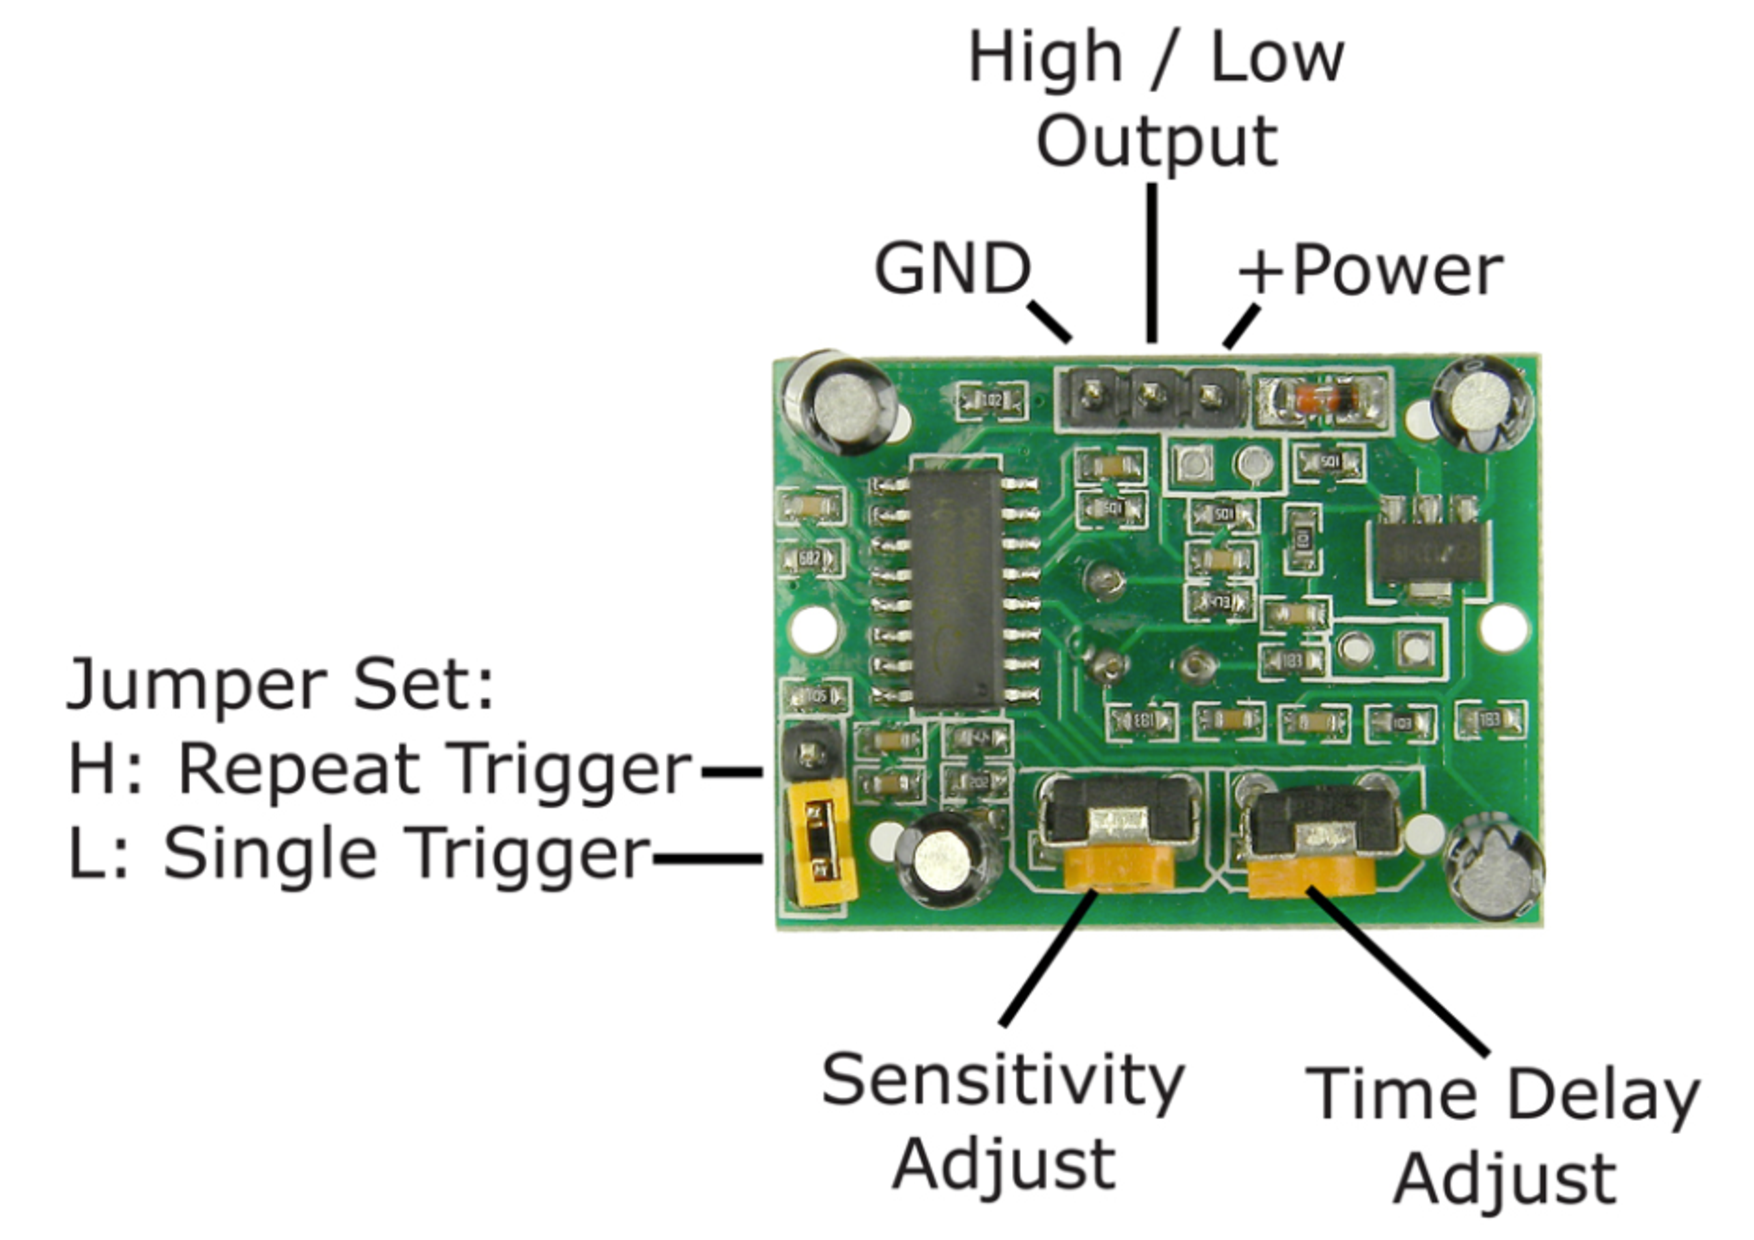
\includegraphics[width=0.5\textwidth]{filer/design/Billeder/pir_overview}}
\caption{Billede af PIR-printet og dets indstillingsmuligheder}
\label{lab:pir_overview}
\raggedright
\end{figure}

\subsection*{Driver}

Driveren der skal drive PIR-sensoren på Enhed skal kunne registrere bevægelse via en get-metode der returnere 1(høj) ved bevægelse og 0(lav) ved stilstand.

\subsubsection*{Pseudokode}

\begin{lstlisting}[language=C]
CY_ISR(PIR){
    Call movement method here
} 

Init interrupt(PIR) on PIR-pin

for(;;){
Detect HIGH(1) on PIR-pin
}
\end{lstlisting}